%
% copied from: https://tikz.net/spherical_volume/
% date: 2023, June 26
%
% adjusted by Alexander Smolka
%
\documentclass[crop,tikz]{standalone}
\usepackage{tikz}
	\usetikzlibrary{shapes}
	\usetikzlibrary{automata}
	\usetikzlibrary{arrows}
	\usetikzlibrary{backgrounds}
	\usetikzlibrary{calc}
	\usetikzlibrary{positioning}
	\usetikzlibrary{patterns}
	\usetikzlibrary{decorations.pathmorphing}
	\usetikzlibrary{decorations.pathreplacing}

\usepackage{siunitx}
\usepackage[version=4]{mhchem}


\input{../../../../resources/latex/_symbols.qmd}

\begin{document}

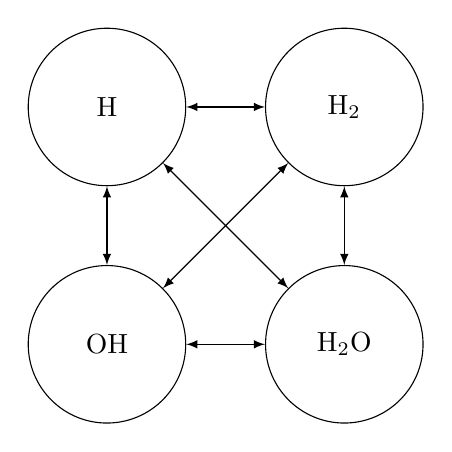
\begin{tikzpicture}[scale=1]

    %::.
    \node[draw, circle, fill=white, inner sep=10pt, minimum size=2cm] (H) at (0,0) {\ce{H}};
    \node[draw, circle, fill=white, inner sep=10pt, minimum size=2cm, right = of H] (H2) {\ce{H2}};
    \node[draw, circle, fill=white, inner sep=10pt, minimum size=2cm, below = of H] (OH) {\ce{OH}};
    \node[draw, circle, fill=white, inner sep=10pt, minimum size=2cm, right = of OH] (H2O) {\ce{H2O}};

    %::.
    \draw[latex-latex] (H) -- (H2);
    \draw[latex-latex] (H) -- (OH);
    \draw[latex-latex] (H) -- (H2O);
    \draw[latex-latex] (H2) -- (OH);
    \draw[latex-latex] (H2) -- (H2O);
    \draw[latex-latex] (OH) -- (H2O);


\end{tikzpicture}

\end{document}